\chapter{Algorithm for test}
\label{cha:bacAlg}

\section{Genetic Algorithm}
\label{subsec:evolutionay_algorithms}
Evolutionary Algorithms are the technique inspired on biological evolution process,
it aims to select the best inviduals that adapt themselves in the environment. For
this adptation is used biological mechanisms such as \textbf{reproduction}, \textbf{mutation},
\textbf{recombination or crossover} and \textbf{selection}. One the most known
evolutionary algorithms is the Genetic Algorithm, it is closely related to evolution
process.

The Genetic Algorithm work on the gene level, so all changes are done in this level.
Although the gene seem to be one component without much relevance, changes done
its can be crucial for adptation in the environment, i.e., the genetic changes
can be crucial to survival of one entire population of individuals or even mean
survival of a species. Rosenzweig~\cite{rosenzweig:1995} cites that in the evolution
process barriers may exist, like geographical barrier retricts gene flow within
a sexually reproducing population and these genes could define the existence another
population.

The Genetic Algorithm process describe in Figure~\ref{fig:ga} has its main strategy
based in tree biological mechanisms: \textbf{reproduction}, \textbf{crossover}
and \textbf{mutation} which are further detailed below:

\begin{itemize}
	\item \textbf{Reproduction}: copies the individuals to participe of the next
	stage (the crossover), they are chosen as their abilities in adapt themselves
	in the environment, those abilities can be calculated according with a function
	\textit{F(x)} that is called as the fitness of the individual like described
	in Figure~\ref{fig:ga}. The copy ratio of the individual is based in your fitness,
	the choise is similar spinning a wheel where each invidual receive slots according
	with your fitness. Thus the individual fitness is greater, then your number
	of copies tends to be greater.

	\item \textbf{Crossover}: the crossover is similar the natural process called
	chromosomal crossover, this process is basead on genetic recombination of
	chromosomes	that produce new genetic combinations. Basically the genetic pair
	of two individuals are combined to generate another genetic pair to resultant
	individual, so the new individual has some characteristics of both parent.
	More minutely in the genetic algorithm two individuals are chosen randomly {\bf(A, B)},
	an integer k, between 0 and the size {\it n} of an individual less one, is chosen
	randomly. The new individual {\it A'} is composed by the first {\it k} genes of A
	and the last {\it k - n} genes of B. The individual {\it B'} consists of the
	first {\it k} genes of B and the last {\it k - n} genes of A. 

	\item \textbf{Mutation}: after the crossover stage one mutation occur in the
	genes of new individuals. The process is simple in which one or more genes are
	selected randomly and then are changed (e.g.change one nucleotide of the DNA
	of one chromosome, or one gene is constituted for bits 0 or 1 and one bit is
	changed from 0 to 1).
\end{itemize}

\begin{figure}[htbp]
	\centering
	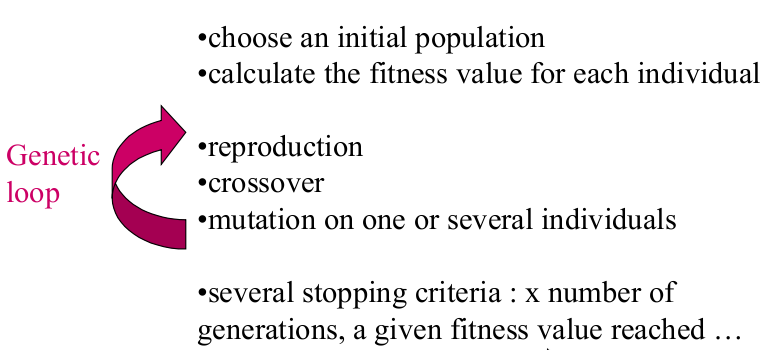
\includegraphics[width=\columnwidth]{img/ga.png}
	\caption{Genetic Algotithm process - Figure extracted of~\cite{baudry}.}\label{fig:ga}
\end{figure}

The algorithm begins with an initial population, for each individual is calculated
your fitness that is the base for reproduction mechanism, so the three biological
mechanisms is called in the specific order already detailed and so the resultant
population is evaluated as one or more criteria, if necessary the three mechanism
are run again and the process continues until the criteria to be achieved.

\section{Bacteriological Algorithm}

Now in the Bacteriological Algorithm(BA) the individual is one bacteria and the focus
of the algorithm is to adapt itself in a given specific environment. The algotithm
is inspired on Genetic Algorithm(GA), but it have some peculiarities that improve
some issues involving the GA and change your behavior.

The BA is more one adaptive approach of GA than one otimization, it introduces a
new mechanism called memorization that is responsable to memorize the best individuals
created along of the generations. As described in ~\cite{baudry} it was proposed
to improve the convergence of the GA, the introduction of the new mechanism might
appear one small modification, but is actually reflect one crucial change of idea
about GA.

Besides of the introduction the new mechanism, the old mechanism crossover was
removed because of the bacteria behavior on its adaptation process in the
environment. This mechanism cannot be used anymore, in terms of natural bacteriologic
process the remotion of the crossover make sense, the bacteria reproduce themself
asexually, the reproduction process consist in duplication of DNA and an after
division to form two new cells.

The algorithm in high-level of abstraction is described in Figure~\ref{fig:ga},
it is fed for one initial population of bacteria, after the bacteriological loop
is started and has four main mechanisms: {\bf Fitness computation}, {\bf Memorization},
{\bf Reproduction} and {\bf Mutation} which are further detailed below:

\begin{itemize}
	\item Fitness computation: the fitness analogously in GA is one way to 	
	differentiate the abilities of each individual in adapt themselves in the
	environment, its calculation depends of one or several criteria defined for 
	the programer and it is used to select the best individuals for the next generation.

	\item Memorization: is the main mechanism introduced by the BA. Its is responsable
	for memorizing the best individuals generated in the process of adaptation,
	as the process continues the population improve more quickly our capacity of
	adaptation. The process consist in memorize the best individuals through of 
	the	generations, if one generation generate bad individuals i.e. generate low
	fitness values, then the memorization operator can ignore this generation and
	use the best individuals already generated in the past to the next generation,
	so avoid regressions in the process.

	\item Reproduction: is similar in GA, the best individuals are sorted ramdomly
	and they are selected to the mutation process. One important point can arise
	in this stage, the population size can grow up exponentially, so thresholds
	must be established.

	\item Mutation: this stage is responsible for generate new individuals, one
	or several genes are changed in order to improve the adaptation of the bacteria
	population in the environment. These new individuals are evaluated by their
	fitness values and they may or may don't be inserted in the set of best
	individuals.

\end{itemize}

\begin{figure}[htbp]
	\centering
	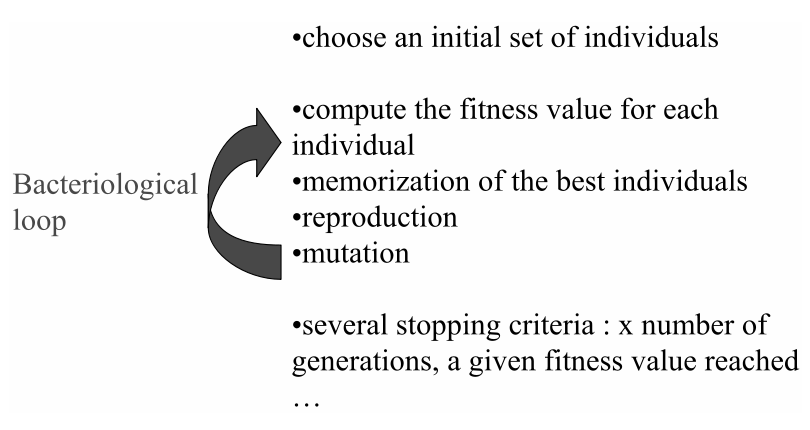
\includegraphics[width=\columnwidth]{img/ba.png}
	\caption{Bacteriological Algotithm process - Figure extracted of~\cite{baudry}.}\label{fig:ba}
\end{figure}

